%%%%%%%% ICML 2021 EXAMPLE LATEX SUBMISSION FILE %%%%%%%%%%%%%%%%%

\documentclass{article}

% Recommended, but optional, packages for figures and better typesetting:
\usepackage{microtype}
\usepackage{graphicx}
\usepackage{subfigure}
\usepackage{booktabs} % for professional tables
\usepackage{stackengine}
\usepackage{amsmath}
\usepackage{amsfonts}
\usepackage{algorithm}
\usepackage{graphicx}
% \usepackage{booktabs}
\usepackage{multirow}
\usepackage{amsmath,bm}
\usepackage{todonotes}



% \usepackage{algpseudocode}


% hyperref makes hyperlinks in the resulting PDF.
% If your build breaks (sometimes temporarily if a hyperlink spans a page)
% please comment out the following usepackage line and replace
% \usepackage{icml2021} with \usepackage[nohyperref]{icml2021} above.
\usepackage{hyperref}

% Attempt to make hyperref and algorithmic work together better:
\newcommand{\theHalgorithm}{\arabic{algorithm}}
\newcommand{\differential}{{\rm{d}}}
\newcommand{\bx}{{\bm{x}}}
\newcommand{\by}{{\bm{y}}}
% Use the following line for the initial blind version submitted for review:
\usepackage{icml2021}

% If accepted, instead use the following line for the camera-ready submission:
%\usepackage[accepted]{icml2021}

% The \icmltitle you define below is probably too long as a header.
% Therefore, a short form for the running title is supplied here:
\icmltitlerunning{Submission and Formatting Instructions for ICML 2021}

\begin{document}

\twocolumn[
\icmltitle{Computational Mean Field Learning}

% It is OKAY to include author information, even for blind
% submissions: the style file will automatically remove it for you
% unless you've provided the [accepted] option to the icml2021
% package.

% List of affiliations: The first argument should be a (short)
% identifier you will use later to specify author affiliations
% Academic affiliations should list Department, University, City, Region, Country
% Industry affiliations should list Company, City, Region, Country

% You can specify symbols, otherwise they are numbered in order.
% Ideally, you should not use this facility. Affiliations will be numbered
% in order of appearance and this is the preferred way.
\icmlsetsymbol{equal}{*}

\begin{icmlauthorlist}
\icmlauthor{Aeiau Zzzz}{equal,to}
\icmlauthor{Bauiu C.~Yyyy}{equal,to,goo}
\icmlauthor{Cieua Vvvvv}{goo}
\icmlauthor{Iaesut Saoeu}{ed}
\icmlauthor{Fiuea Rrrr}{to}
\icmlauthor{Tateu H.~Yasehe}{ed,to,goo}
\icmlauthor{Aaoeu Iasoh}{goo}
\icmlauthor{Buiui Eueu}{ed}
\icmlauthor{Aeuia Zzzz}{ed}
\icmlauthor{Bieea C.~Yyyy}{to,goo}
\icmlauthor{Teoau Xxxx}{ed}
\icmlauthor{Eee Pppp}{ed}
\end{icmlauthorlist}

\icmlaffiliation{to}{Department of Computation, University of Torontoland, Torontoland, Canada}
\icmlaffiliation{goo}{Googol ShallowMind, New London, Michigan, USA}
\icmlaffiliation{ed}{School of Computation, University of Edenborrow, Edenborrow, United Kingdom}

\icmlcorrespondingauthor{Cieua Vvvvv}{c.vvvvv@googol.com}
\icmlcorrespondingauthor{Eee Pppp}{ep@eden.co.uk}

% You may provide any keywords that you
% find helpful for describing your paper; these are used to populate
% the "keywords" metadata in the PDF but will not be shown in the document
\icmlkeywords{Machine Learning, ICML}

\vskip 0.3in
]

% this must go after the closing bracket ] following \twocolumn[ ...

% This command actually creates the footnote in the first column
% listing the affiliations and the copyright notice.
% The command takes one argument, which is text to display at the start of the footnote.
% The \icmlEqualContribution command is standard text for equal contribution.
% Remove it (just {}) if you do not need this facility.

%\printAffiliationsAndNotice{}  % leave blank if no need to mention equal contribution
\printAffiliationsAndNotice{\icmlEqualContribution} % otherwise use the standard text.

\begin{abstract}
 The mean field interpretations of learning dynamics in over-parameterized neural networks have appeared in recent years, and offered theoretical insights on the empirical success of first order optimization algorithms in finding global minimum of the nonconvex risk landscape. In this work, we explore transcending the mean field learning dynamics from a theoretical tool to a computational algorithm. We design Sinkhorn regularized proximal algorithms to approximate the distributional flow generated by the learning dynamics in the mean field regime over weighted point clouds. The time-varying weights are computed via certain contractive fixed point recursion. This numerically realizes the interacting Wasserstein gradient flow of the parameter distribution supported over the neuronal ensemble. We implement the proposed computational framework of interacting weighted particle evolution for classification and GAN. For training the classifier, the proposed algorithm performs gradient descent of the free energy associated with the risk functional. For training the GAN, the proposed algorithm performs gradient descent-ascent for finding the mixed-strategy Nash equilibrium. We provide detailed numerical results to illustrate the proposed computational framework.
\end{abstract}

\section{Introduction}
\label{introduction}
TBD
\section{Equations}

\begin{equation}
\label{phi}
    \varphi(\underline{\bx},\underline{\bm{\bm{\theta}}}_{i})=a_{i} \sigma(\langle \underline{w}_{i},\underline{\bx} \rangle +b_i))
\end{equation}
 where $\sigma$ is activation function, $\underline{\bx} \in \mathbb{R}^{n_{x}}$ is the features vector and $a_{i}$, $\underline{\bm{w}}_{i}$, and $b_{i}$ ($i$ runs from 1 to $N$, number of samples) are scaling, weight, and bias parameters, respectively. 
 
  $$\underline{\bm{\bm{\theta}}}=\begin{pmatrix} \underline{\bm{\bm{\theta}}}_{1}\\ \underline{\bm{\bm{\theta}}}_{2}\\ 
 \vdots\\
 \underline{\bm{\bm{\theta}}}_{N}\end{pmatrix} \in \mathbb{R}^{(n_{x}+2)\times N}~~ \text{where}~~  \underline{\bm{\bm{\theta}}}_{i}=\begin{pmatrix} a_{i}\\ b_{i}\\ \underline{\bm{w}}_i\end{pmatrix} \in \mathbb{R}^{n_{x}+2}
$$
 
\begin{subequations}
\begin{align}
 \widehat{f}(\underline{\bx},\underline{\bm{\bm{\theta}}})&=\int_{\mathbb{R}^{n_p}} \varphi(\underline{\bx},\underline{\bm{\bm{\theta}}}) \differential \mu (\underline{\bm{\bm{\theta}}}) \\
    & =\int_{\mathbb{R}^{n_p}} \varphi(\underline{\bx},\underline{\bm{\bm{\theta}}}) \varrho(\underline{\bm{\bm{\theta}}}) \differential \underline{\bm{\bm{\theta}}}] \label{f_hat_weight} \\  
      &= \mathbb{E}_{\underline{\bm{\bm{\theta}}}} \left[ \varphi(\underline{\bx},\underline{\bm{\bm{\theta}}})\right] \label{f_hat_average}
\end{align}
\label{f_hat}
\end{subequations}

\begin{equation}
    \underline{\bm{\theta}}_{k}^{i}=\underline{\bm{\theta}}_{k-1}^{i}-h \nabla \left( U(\underline{\bm{\theta}}_{k-1}^{i})+V (\underline{\bm{\theta}}_{k-1}^{i}) \right)+\sqrt{2 \beta^{-1}}...
    \label{EulerMaruyama}
\end{equation}


\begin{algorithm}
\caption{Algorithm1}\label{alg1}
TBD
\end{algorithm}


\section{Experiments}
\label{Experiments}
We evaluate the proposed computational framework on two real-world datasets. All numerical experiments are performed on a PC with 3.4 GHz  6-Core Intel Core i5 processor, and 8 GB RAM. The codes are publicly available at

\href{https://github.com/inodozi/ICML-2022-paper-Git-repo/tree/main/Codes}{https://github.com/inodozi/ICML-2022-paper-Git-repo/tree/main/Codes}

\color{red}TBD\color{black}
% In the following subsection, we will present the results from implementing the proposed computational framework to the Wisconsin diagnostic breast cancer (WDBC) datasets. This experiment took about 33 hours of computation. 
\subsection{WDBC Dataset}\label{subsec.WDBC}
In this experiment, we perform a binary classification case study with quadratic loss using the Wisconsin diagnostic breast cancer (WDBC) dataset from the UC Irvine machine learning repository \cite{Dua:2019}. For this dataset, $n_{\text{data}} = 569$, and the number of features $n_x=30$. The label $0$ (resp. $1$) denotes ``benign" (resp. ``malignant"). The WDBC dataset has 357 instances as ``benign" and 212 instances as ``malignant".

For implementing Algorithm \ref{alg1} to the above dataset, we set $\varrho_{0} \equiv \text{Unif}\left( [0.9, 1.1]\times [-0.1, 0.1] \times [-1,1]^{n_{x}}\right)$, a uniform joint density function supported over $n_{p}=n_{x}+2=32$ dimensional mean field parameter space.

We generate $N=1000$ i.i.d. samples from $\varrho_{0}$, and set the tolerance $\delta=10^{-3}$ and the maximum number of iterations $L=300$. Then, we apply the proposed proximal recursion to \eqref{EulerMaruyama} with time step $h=10^{-3}$, and the regularization parameter $\varepsilon=1$. To calculate the gradients of the functions $U$ and $V$ in \eqref{EulerMaruyama}, we use the automatic differentiation module of PyTorch Library \cite{paszke2017automatic}. 

We used 70\% of the entire dataset for learning the mean field parameter distribution via weighted scattered point cloud evolution using the proximal recursions. Then, we use the confusion matrix method \cite{visa2011confusion} to evaluate the accuracy of the obtained model for the test data ($30 \%$  of the entire dataset).

  The activation function in \eqref{phi}, is  $\sigma=\tanh$. We calculate $\varphi(\underline{\bx},\underline{\bm{\theta}})$ in \eqref{phi} where $\underline{\bm{\theta}}$ is obtained from training process and $\underline{\bx}$ is the test data. We estimate $\widehat{f}$ in \eqref{f_hat} in two ways. First, we estimate $\widehat{f}$ as a sample average of $\varphi$. Second, we estimate $\widehat{f}$ by numerically approximating the integral in \eqref{f_hat_weight} using the propagated samples $\{ \bm{\theta}_{k}^{i},\varrho_{k}^{i}\}_{i=1}^{N}$ for $k\in\mathbb{N}$. The difference between the two estimates is that the first is an empirical average while the second uses the weights $\{\varrho_{k}^{i}\}_{i=1}^{N}$ obtained from the proposed proximal algorithm. We refer to these as the ``estimate \#1" and ``estimate \# 2", respectively. The $\widehat{f}$ estimates thus obtained, are then passed through a softmax (for estimate \#1) and argmax (for estimate \#2) functions, to get the predicted labels. 

We run the simulation for different values of the inverse temperature $\beta$, and list the corresponding classification accuracy in Table\ref{tab:accuracy}. For each fixed $\beta$, we perform $10^{6}$ proximal recursions incurring approx. 33 hours of computational time. Fig. \ref{fig_f_hat_and_labels} compares the predicted labels with the actual labels, for the two methods. 

\begin{table}[h!]
\centering
 \begin{tabular}{|c c c|} 
 \hline
  \multicolumn{3}{|c|}{Classification accuracy for the WBDC dataset} \\
 \hline\hline
 $\beta$ & Estimate \#1 & Estimate \#2  \\  
 \hline
 0.03  & $91.17\%$ & $92.35\%$\\
 0.05&    $92.94 \%$ &  $92.94 \%$   \\
 0.07 &$78.23\%$ & $92.94\%$\\
 \hline
 \end{tabular}
     \caption{Classification accuracy of the proposed computational framework for the WBDC dataset with different values of the inverse temperature $\beta$.}
    % \label{tab:accuracy}
\label{tab:accuracy}
\end{table}


% \begin{table}[h]
%     \begin{center}
% \begin{tabular}{ |p{2cm}||p{2cm}|p{2cm}|  }
%  \hline
%  \multicolumn{3}{|c|}{Classification accuracy for the WBDC dataset} \\
%  \hline
% $~~~\beta$&Estimate \#1 & Estimate \#2\\
%  \hline
%  0.03  & $91.17\%$    & $92.35\%$\\
%  0.05&    $92.94 \%$   &  $92.94 \%$   \\
%  0.07 &$78.23\%$ & $92.94\%$\\
%  \hline
% \end{tabular}
% \end{center}
%     \caption{Accuracy of the proposed computational framework for different value of inverse temperature $\beta$ implementing for the WBDC dataset.}
%     % \label{tab:accuracy}
% \end{table}

\begin{figure}[h]
\centering
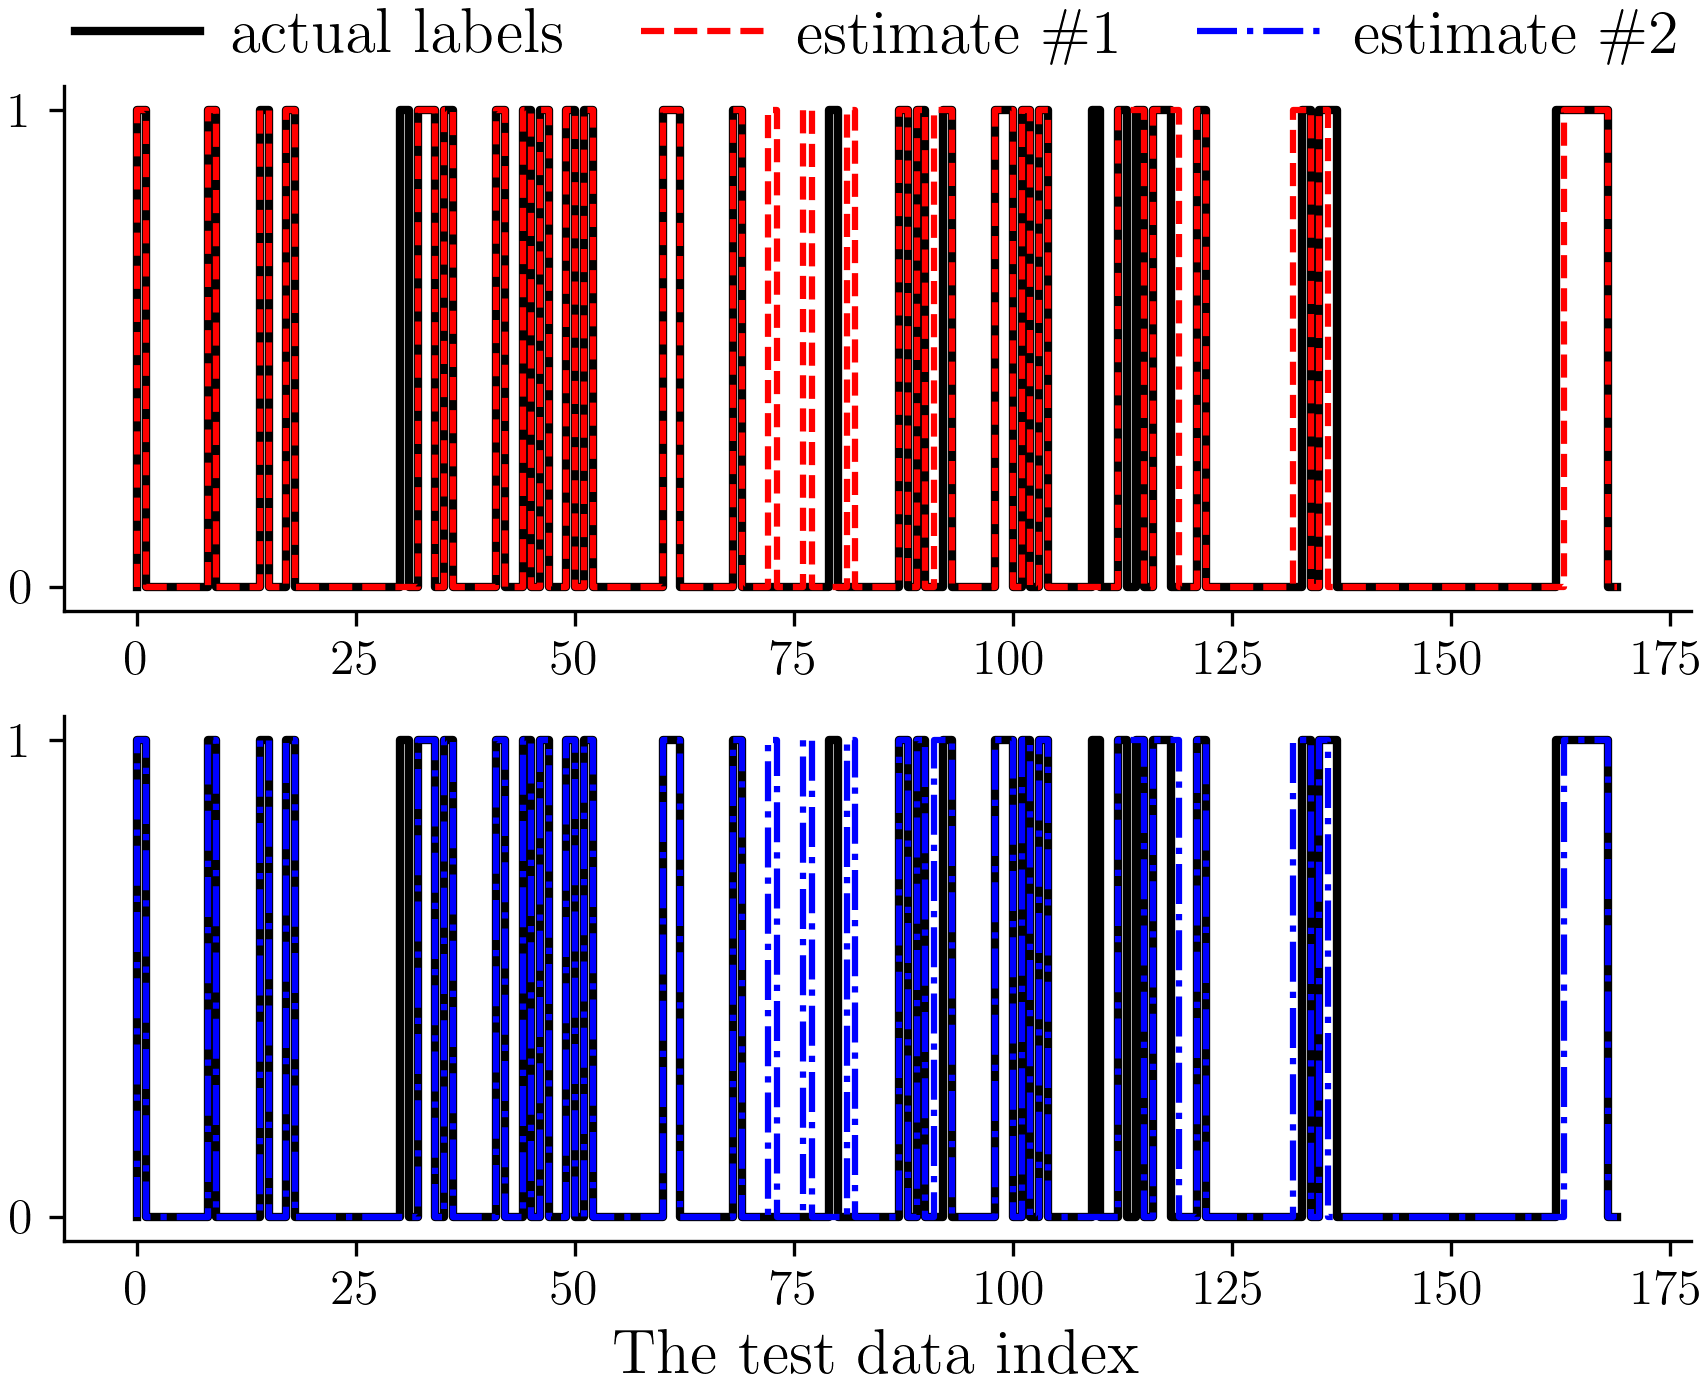
\includegraphics[width=0.45\textwidth]{f_hat_WBDC.png}
\caption{Comparison of the predicted labels with the actual labels for the test data of WBDC dataset with $\beta=0.05$. Top: comparison of the labels for estimate \#1. Bottom: the same for estimate \#2.}
\label{fig_f_hat_and_labels}
\end{figure}
\begin{figure}[h]
\centering
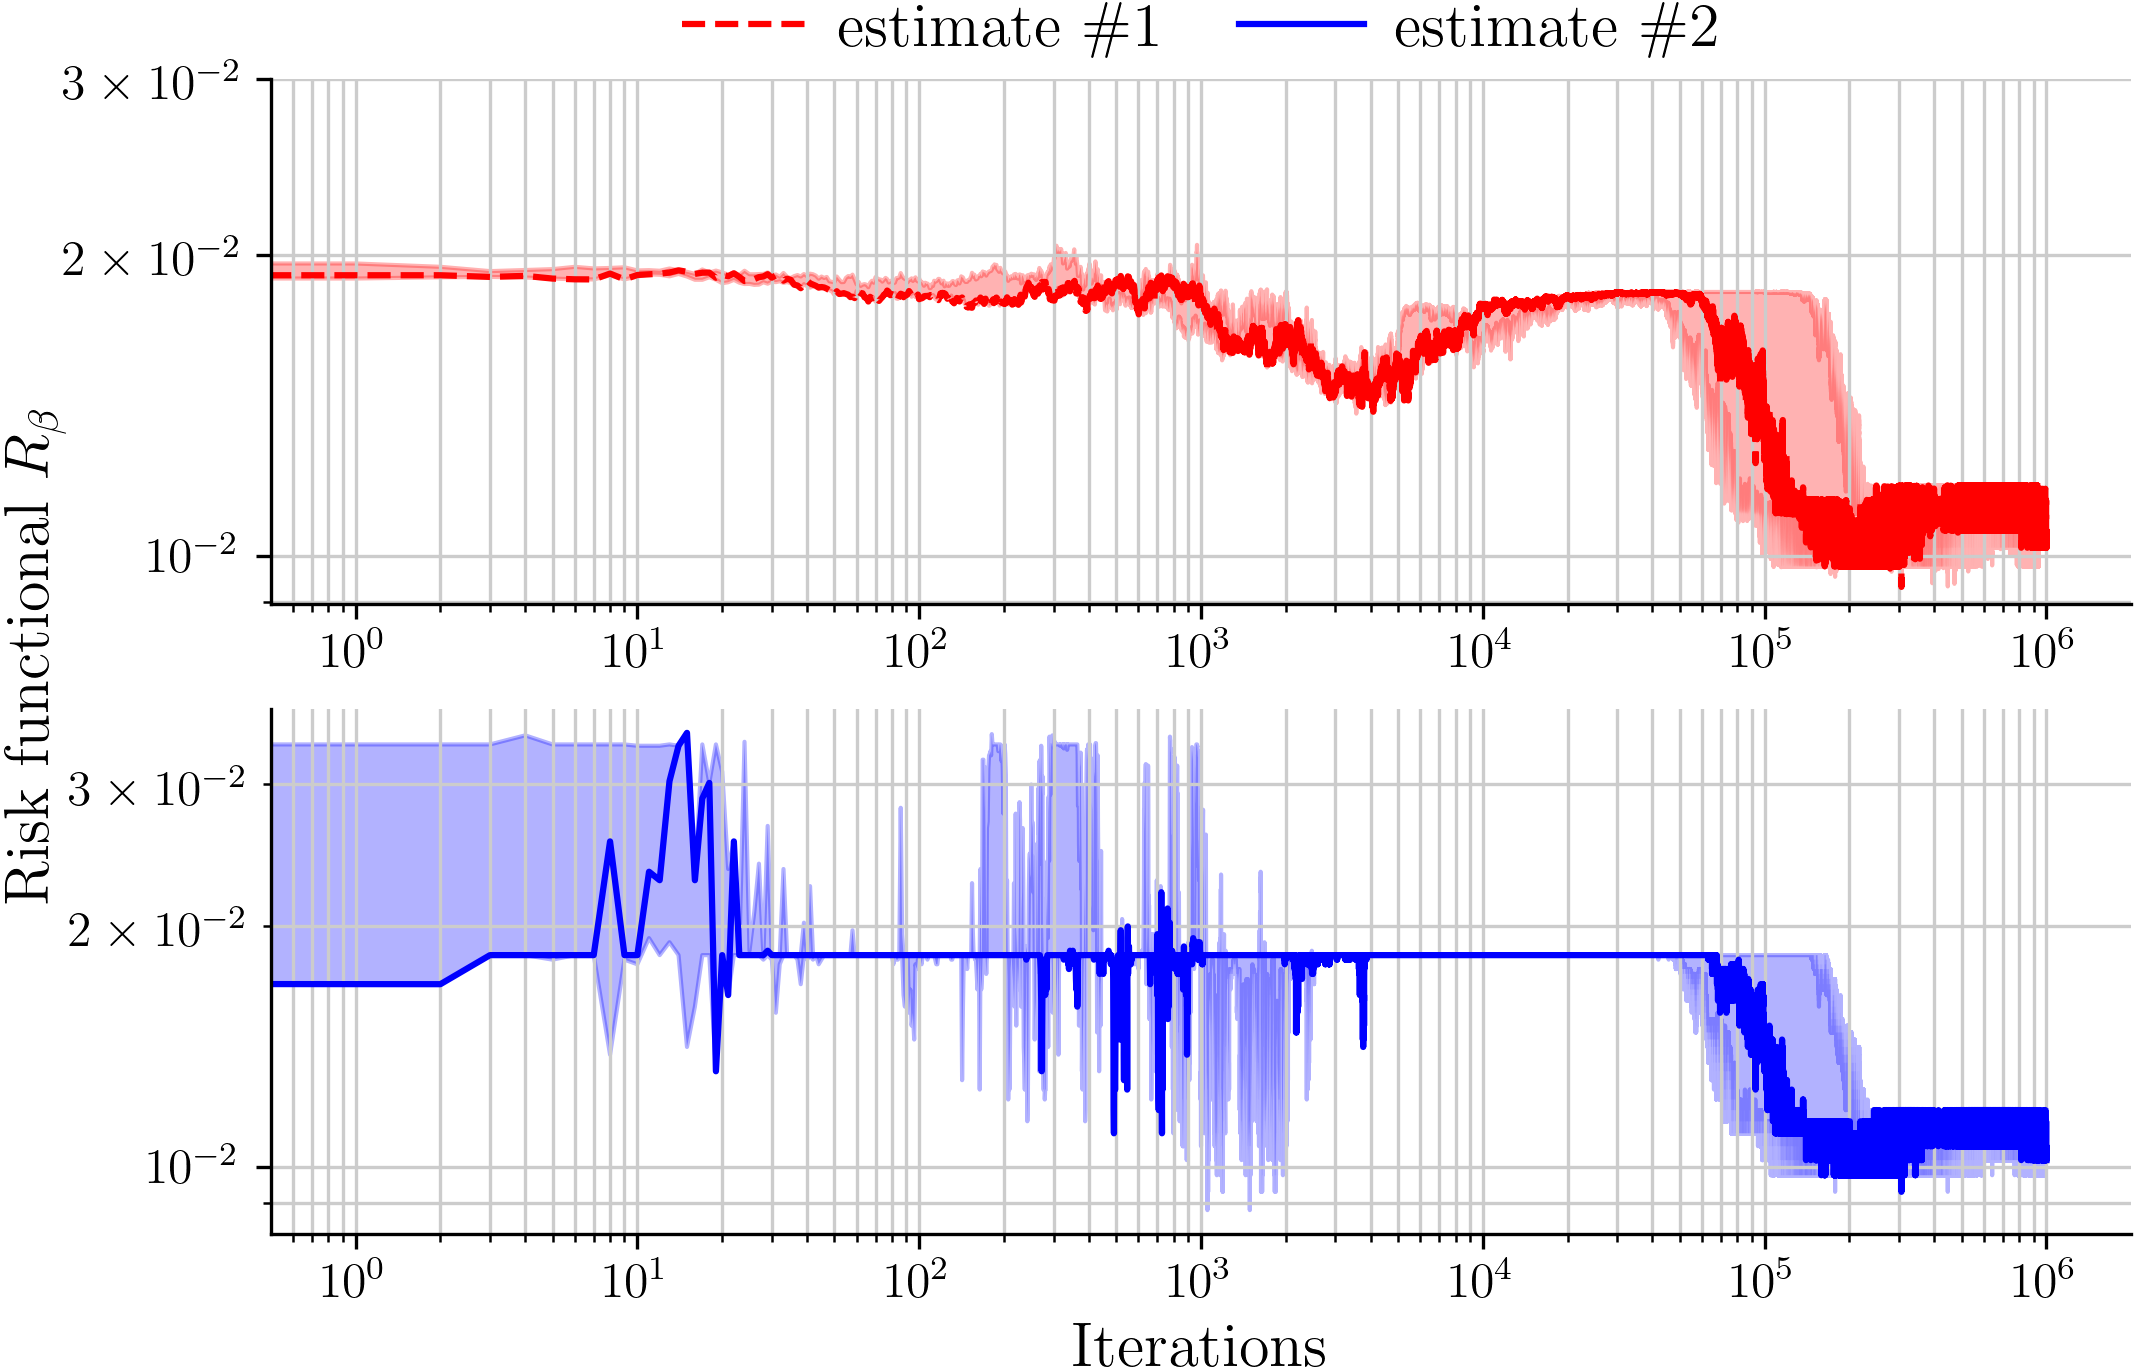
\includegraphics[width=0.45\textwidth]{Risk_WBDC.png}
\caption{Risk functional $R_{\beta}$ versus the number of proximal recursions shown for the WBDC dataset with $\beta=0.05$. The shadow shows the Risk functional variation range for different values of beta ($0.03,0.05,0.07$).}
\label{fig_risk}
\end{figure}
Fig. 2 shows the risk functional, computed as the averaged loss over the test data using the two estimates mentioned before.
\subsection{MNIST Dataset}
In the second experiment, we perform a digit classification case study with quadratic loss using the benchmark dataset Modified National Institute of Standards and Technology (MNIST) \cite{lecun1998gradient}. For this dataset, $n_{\text{train data}} = 60000$, and $n_{\text{test data}} = 10000$. All images are of size $28 \times 28$ so the number of features $n_x= 28 \times 28 =784$. Each image has assigned a label from the range $[0-9]$.

Before implementing Algorithm \ref{alg1} to the above dataset, we use an autoencoder developed with the Keras library to reduced the dimension of our data to $n_x = 64$ \cite{keras}. 

The parameters ($N$, $\varrho_0$, $\delta$, $L$, $h$, $\epsilon$, and $\sigma$) are chosen the same as subsection \ref{subsec.WDBC}.
Also, to calculate the gradients of the functions $U$ and $V$ in \eqref{EulerMaruyama}, we use the automatic differentiation module of PyTorch Library.
The results reported for a latent space of dimension $n_x = 64$.

We used training dataset for learning the mean field parameter distribution via weighted scattered point cloud evolution using the proximal recursions. Then, we use the confusion matrix method \cite{visa2011confusion} to evaluate the accuracy of the obtained model for the test data.


Here the gradients of the functions $U$ and $V$ in \eqref{EulerMaruyama} with respect to $\theta$ is obtained over a mini-batch with size of $1000$ via automatic differentiation module of PyTorch Library. Using this approximation of drift, we then updated the weights and the joint PDF as we did in the case of WDBC.

 The results will be shown in Fig \ref{fig_f_hat_MNIST}, \ref{fig_risk_MNIST} and table \ref{tab:accuracy_MNIST} \color{black}


\begin{table}[h!]
\centering
 \begin{tabular}{|c c|} 
 \hline
  \multicolumn{2}{|c|}{Classification accuracy for the MNIST dataset} \\
 \hline\hline
 $\beta$ & Accuracy   \\  
 \hline
 ...  & $...\%$ \\
 ...&    $... \%$  \\
 ... &$...\%$ \\
 \hline
 \end{tabular}
     \caption{Classification accuracy of the proposed computational framework for the MNIST dataset with different values of the inverse temperature $\beta$.}
    % \label{tab:accuracy}
\label{tab:accuracy_MNIST}
\end{table}



\begin{figure}[h]
\centering
\noindent\includegraphics[scale=0.5]{example-image-c} 
\caption{Comparison of the predicted labels with the actual labels for the test data of MNIST dataset.}
\label{fig_f_hat_MNIST}
\end{figure}

\begin{figure}[h]
\centering
\noindent\includegraphics[scale=0.5]{example-image} 
\caption{Risk functional $R$ versus the number of proximal recursions shown for the MNIST test dataset.}
\label{fig_risk_MNIST}
\end{figure}


\clearpage
\bibliography{ref}
\bibliographystyle{icml2021}


\end{document}


